\chapter{Részecske-raj optimalizáció}

Ebben a fejezetben a részecske-raj optimalizáció kerül bemutatásra.

\section{Rajintelligencia}

Az állatok alapvető túlélési ösztönei közé tartozik az élelem és élőhely utáni keresés. Ez minden állatfajra igaz, a hangyától a bálnáig, mégis a csoportokban élő állatfajok különösen egymásra vannak utalva ilyen téren. Az oka ennek, hogy külön-külön valószínűleg elpusztulnának, de csoportokban sokkal erősebbek és védettebbek lesznek. Ezt a jelenséget nevezik \textit{rajintelligenciának} \index{rajintelligencia}, miszerint a nem-intelligens egyedek intelligens viselkedésmintákat mutatnak csoportokban, ami végül sikeres túlélési képességet eredményez \parencite{rapaic2019}.

1995-ben James Kennedy amerikai pszichológus és Russel C. Eberhart mérnök pontosan definiálták ezeket a viselkedésmintákat, és így született meg a részecske-raj optimalizáció \parencite{dorigo2007}.

\section{A részecske-raj optimalizáció alapjai}

A részecske-raj optimalizációs algoritmus \index{részecske-raj algoritmus} populációja olyan egyedekből áll, amelyek állandó mozgásban tartják az egész rajt. Ez a mozgás nagyban függ az egyed saját tapasztalataitól, vagyis az eddigi bejárt úttól. Az így megszerzett információk alapján az egyedek egymással kommunikálnak, és a lehető legjobb eredmény felé mozdulnak el. Ez a mozgás ciklusonként frissül, ami a gyakorlatban annyit jelent, hogy lépésenként változik a raj helyzete. A genetikus algoritmustól eltérően a populáció tagjai nem cserélődnek, mindig ugyanazok az egyedek szerepelnek a rajban, csak a helyzetük változik.

Ha a sorrendben $n$-edik ciklus keresztmetszetét vesszük, minden részecske a következő információkat hordozza magával:

\begin{itemize}
    \item a részecske jelenlegi helyzete -- $x[n]$:
a keresési tartomány egyik értéke, dimenzionalitása függ a kritériumfüggvény dimenziójától;
	\item jelenlegi sebesség -- $v[n]$:
a részecske előző lépésből szerzett sebessége (az előző helyzettől való elmozdulása);
	\item a részecske eddigi legjobb helyzete -- $p[n]$:
a részecskének az a pozíciója, amelyet eddigi útja során felvett, és a legjobb értéket hordozza.
\end{itemize}

A fent említett paraméterek mellett fontos még a raj szintjén történő információcsere, vagyis a raj szintjén elért eddigi legjobb helyzet -- $g[n]$. Ez a paraméter a valaha elért legjobb részecske helyzetét jelenti.

A részecskék térben és időben történő változását a \ref{eq:vn} és a \ref{eq:xn} egyenletek határozzák meg.

\begin{equ}[!ht]
  \begin{equation}
    v[n+1] = w \cdot v[n] + cp \cdot rp[n] \cdot (p[n]-x[n]) + cg \cdot rg[n] \cdot (g[n] - x[n])
  \end{equation}
  \caption{\label{eq:vn}}
  \begin{equation}
    x[n+1] = x[n] + v[n+1]
  \end{equation}
  \caption{\label{eq:xn}}
\end{equ}

Az $rp[n]$ és az $rg[n]$ egymástól független véletlenszerű számok $0$ és $1$ között, míg a $w$, $cp$ és $cg$ együtthatók alkotják az algoritmus komponenseit:

\begin{itemize}
    \item inerciális komponens -- $w \cdot v[n]$:
az előző lépésben kiszámolt sebességet befolyásoló $w$ együttható egy részecske szabad mozgását szimulálja, vagyis nagyobb teret ad a részecske szabad mozgásának;
	\item kognitív komponens -- $cp \cdot rp[n] \cdot (p[n]-x[n])$:
$cp$ gyorsulási együttható meghatározza, hogy egy részecske eddigi tapasztalatai mennyire befolyásolják a részecske következő helyzetét;
	\item szociális komponens -- $cg \cdot rg[n] \cdot (g[n]-x[n])$:
$cg$ együttható a részecskék együttműködési hajlandóságát határozza meg, vagyis a raj szintjén jelentkező legjobb értékhez történő közelítést biztosítja.
\end{itemize}

\begin{figure}
    \centering
    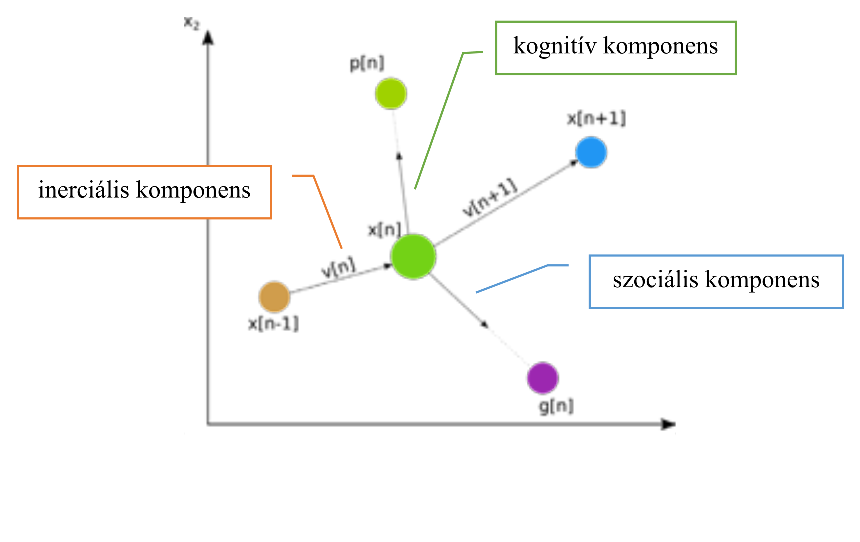
\includegraphics[width=0.8\textwidth]{komponensek}
    \caption{A részecske-raj optimalizáció komponensei \parencite{kanovic2017}}
    \label{fig:komponensek}
\end{figure}

Az algoritmus komponenseinek a kölcsönhatásait a \ref{fig:komponensek} ábra vizualizálja. Az egyes komponensek súlyozott értékei ($w$, $cp$ és $cg$) tetszőlegesen választhatóak, ebből eredendően több változata létezik a részecske-raj algoritmusnak. A dolgozatban bemutatott változatban ezek az együtthatók időben változó értékek, melyeknek az értékei a \ref{tab:psokomp} táblázatban találhatóak meg.

\begin{table}
    \centering
    \begin{tabular}{|c|c|c|}
    \hline
    együttható & kezdő érték & végső érték \\ \hline
    \hline
    $w$ & 0.9 & 0.4 \\ \hline
    $cp$ & 2.5 & 0.5 \\ \hline
    $cg$ & 0.5 & 2.5 \\ \hline
    \end{tabular}
    \caption{Az időben változó együtthatók értéke \parencite{kanovic2017}}
    \label{tab:psokomp}
\end{table}

\section{A részecske-raj algoritmus}

Első lépésként a raj nagyságát kell meghatározni, ami becslések alapján nagyjából tízszerese kell, hogy legyen a probléma dimenziójától \parencite{rapaic2019}. Erre azért van szükség, mert túl kevés egyed képtelen bejárni az egész keresési mező összes dimenzióját és információ hiányában nem kerül felderítésre lehetséges megoldások.

Az algoritmus elején minden részecskéhez véletlenszerűen egy kezdő pozíciót kell rendelni ($x[0]$), ami egyben az egyedek eddigi legjobb pozícióját is jelenti ($p[0]$). A kritériumfüggvény alapján kiszámoljuk melyik pozíció a legjobb, ez lesz a globális legjobb pozíció ($g[0]$). Ezzel lezárult az inicializációs rész.

A fő részben minden részecskének ki kell számolni a következő sebességét -- \ref{eq:vn} képlet, és ez alapján a pozícióját -- \ref{eq:xn} képlet. A részecske eddigi legjobb helyzetét is meg kell változtatni, ha az újabb pozícióra jobb eredmény születik. Miután bejeződött a ciklus, a globális pozíciót kell frissíteni úgy, hogy a részecskék eddigi legjobb pozícióinak az értékét hasonlítjuk össze a globálisan legjobb értékkel.

\linespread{1}
\begin{lstlisting}[caption={A részecske-raj algoritmus pszeudokódja \parencite{dorigo2008}}, captionpos=b]
begin pso-algoritmus
   %(*raj inicializáció*)
   while (%(*leállási feltétel nem teljesített*))
   do
      for (i=1 to %(*részecskék száma*))
         %(*sebesség és az új pozíció kiszámolása*)
         %(*kritériumfüggvény értékének meghatározása*)
         %(*részecske eddigi legjobb pozíciójának a frissítése*)
      end
      %(*globálisan legjobb pozíció frissítése*)
   end do
end pso-algoritmus
\end{lstlisting}

Leállási feltételként leggyakrabban egy előre megadott maximális ciklusszámot használnak, de ez függ a probléma típusától. Egy másik megoldás lehet a globálisan legjobb pozícióra kapott érték változását követni, miszerint ha egy megadott tűréshatár alá esik az érték változása, akkor teljesül a leállási feltétel \parencite{kanovic2017}.

\section{A részecske-raj algoritmus kivizsgálása}

A genetikus algoritmushoz hasonlóan, a részecske-raj algoritmus is demonstratív módon a Rastrigin-féle tesztfüggvény \ref{eq:rastrigin} által kerül elemzésre.

A fent leírt algoritmus alapján és a megfelelő paraméterek segítségével egy sajátkezűleg írt programot készítettem \textit{Python} programnyelvben \parencite{kisspy2020}. A vektorszámításokat a \textit{NumPy} könyvtár segítségével oldottam meg, míg az eredmények grafikonon történő megjelenítéséhez a \textit{matplotlib} könyvtárat használtam. A dolgozatban szereplő Rastrigin-függvény és minden egyéb grafikonos ábra szintén ezzel a szoftverrel készült el.

Az algoritmus elemzése négyféle környezetben zajlott, és mindegyik kísérlet 100-szoros ismétléssel történt. Az eredmények a \ref{tab:psores} táblázatban találhatók meg.

\begin{table}
    \centering
    \begin{tabular}{|c|c|c|c||c|c|c|}
    \hline
    \# & \rotatebox{90}{populációszám} & \rotatebox{90}{ciklusszám} & elhelyezés & átlageredmény & medián & szórás \\ \hline
    \hline
    \textbf{K1} & 25 & 100 & uniform & $0.3283$ & $8.7512 \cdot 10^{-12}$ & $0.4678$ \\ \hline
    \textbf{K2} & 25 & 1000 & uniform & $0.1194$ & $0$ & $0.3233$ \\ \hline
    \textbf{K3} & 25 & 100 & nem-uniform & $0.7960$ & $0.9950$ & $0.9850$ \\ \hline
    \textbf{K4} & 40 & 100 & nem-uniform & $0.3781$ & $1.5721 \cdot 10^{-13})$ & $0.6098$ \\ \hline
    \end{tabular}
    \caption{A részecske-raj optimalizáció elemzésének az eredményei}
    \label{tab:psores}
\end{table}

Az eredményekből egyértelműen látható, hogy az egyenletesen elhelyezkedő populáció esetében a ciklusszám növelése 100-ról 1000-re nem hatott ki az eredmény pontosságára, míg a nem egyenletesen elhelyezkedő populáció esetében a populáció számának a növelése nagyban javított az eredményen. Ez annak köszönhető, hogy az algoritmus komponenseinek az együtthatói időben változnak, így az idő múlásával csökken az egyedek felderítési hajlama, míg a szociális komponens erősödik. Ez azzal jár, hogy a kísérlet végére az egyedek egyre jobban hagyatkoznak az eddigi globálisan elért legjobb eredményre; így ha nem járták be a keresési mezőt, nagy valószínűséggel a legjobb eredmény egy lokális minimumban akad meg. A populáció számának a növelése esélyt ad a keresési mező jobb felderítésére, így megtalálva az optimális értéket.

Az algoritmus vizualizációja érdekében készítettem egy \textit{Javascript} programot, amely bármilyen böngészőből lefuttatható \parencite{kissjs2020}. A Rastrigin-féle függvény mellett még egyéb más tesztfüggvények is elérhetőek, melyekre (a kiválasztott paraméterek mellett) ki lehet számolni az optimális értéket (\ref{fig:psojs1} ábra). A számolás befejeztével megjelenik egy időcsúszkával ellátott grafikon (\ref{fig:psojs2} ábra), ahol végig lehet követni a populáció helyzetét a generációk folyamán. A raj animált mozgásának köszönve szemügyre vehető egy-egy részecske vándorlása valamint az egész populáció szintjén történő együttműködés, viselkedésminta.

\begin{figure}
    \centering
    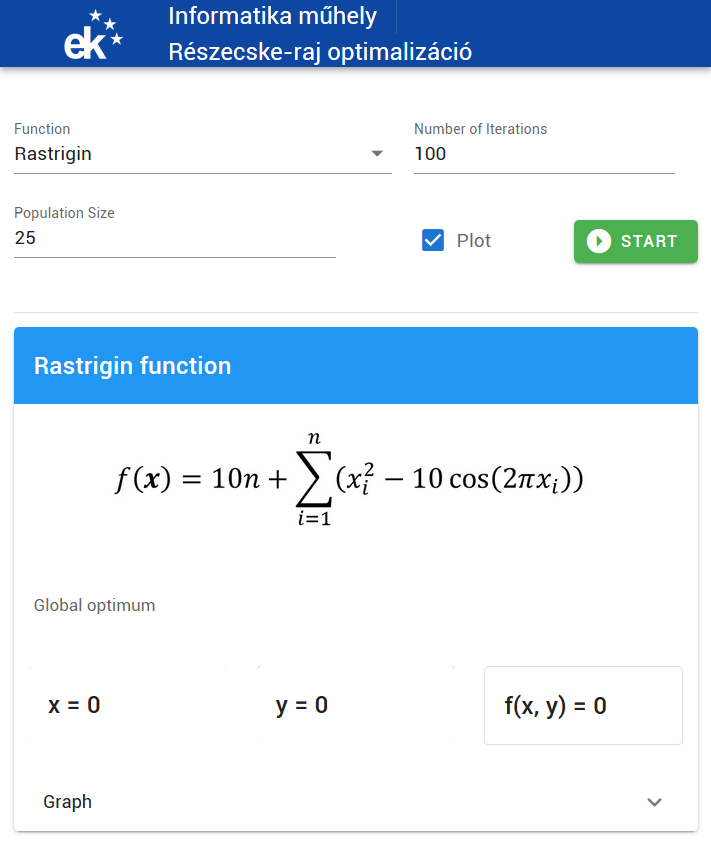
\includegraphics[width=0.6\textwidth]{psojs1}
    \caption{Paraméterek beállítása}
    \label{fig:psojs1}
\end{figure}

\begin{figure}
    \centering
    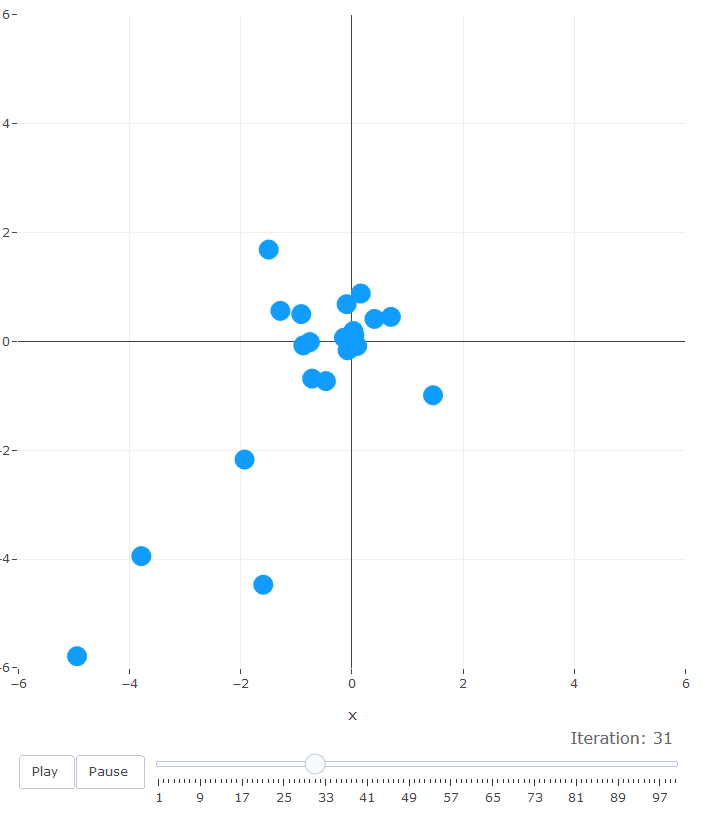
\includegraphics[width=0.6\textwidth]{psojs2}
    \caption{A részecskék időbeli mozgása}
    \label{fig:psojs2}
\end{figure}

\section{A részecske-raj algoritmus felhasználási területei}

Az algoritmus egyszerűségéből fakadóan sok szakterületen megállta a helyét, így pl. az egészségügyben leukémia-típusú problémák diagnózisában. Közgazdasági területen a kockázati befektetések elemzésére használják. Jelentkezik mechanikában, termodinamikában, valamint egyéb geometriai optimalizációs problémáknál is (pl. szenzorok optimális elhelyezése). Az optimális vezérlés, rendszermodellezés, károk észlelése és még sok más gyakorlati problémához kínál megoldást a részecske-raj algoritmus \parencite{almeida2019}.

A gyakorlati problémák mellett elméleti és más absztrakt témához is segítséget nyújt. A mesterséges intelligencia és a gépi tanulás kiképzési folyamatában valamint a mesterséges neuronhálózat paramétereinek optimális értékének a megkeresésében is használják a részecske-raj algoritmust \parencite{kanovic2017}.
